\documentclass[border=5pt]{standalone}
\usepackage{tikz}
\usepackage{amsmath}
\usetikzlibrary{positioning, arrows.meta, calc, fit, backgrounds}

% --- Color Scheme (Blue-Gray) ---
\definecolor{bgPrimary}{HTML}{DAE8FC}
\definecolor{bgSecondary}{HTML}{E8EEF7}
\definecolor{bgAccent}{HTML}{B3CDE3}
\definecolor{bgInput}{HTML}{F0F4F8}
\definecolor{borderPrimary}{HTML}{6C8EBF}
\definecolor{borderAccent}{HTML}{3A6EA5}
\definecolor{arrowColor}{HTML}{4A6A8A}
\definecolor{textMain}{HTML}{2C3E50}
\definecolor{textLight}{HTML}{7F8C8D}
\definecolor{bgHighlight}{HTML}{FFF3CD}
\definecolor{badgeBg}{HTML}{E8EEF7}

% --- Styles ---
\tikzset{
  module/.style={draw=borderPrimary, fill=bgPrimary, rounded corners=4pt,
    minimum width=2.8cm, minimum height=1.2cm,
    font=\sffamily\small, text=textMain, line width=0.6pt, align=center},
  novelmodule/.style={draw=borderAccent, fill=bgAccent, rounded corners=4pt,
    minimum width=2.8cm, minimum height=1.2cm,
    font=\sffamily\small\bfseries, text=textMain, line width=1.0pt, align=center},
  iobox/.style={draw=borderPrimary, fill=bgInput, rounded corners=3pt,
    minimum width=2cm, minimum height=1cm,
    font=\sffamily\small, text=textMain, line width=0.5pt, align=center},
  stdarrow/.style={-{Stealth[length=5pt, width=4pt]}, line width=0.6pt, color=arrowColor},
  srcbox/.style={draw=borderPrimary, fill=bgInput, rounded corners=3pt,
    minimum width=3.6cm, minimum height=0.7cm,
    font=\sffamily\scriptsize, text=textMain, line width=0.5pt, align=left,
    inner xsep=6pt},
  badge/.style={draw=borderPrimary, fill=badgeBg, rounded corners=2pt,
    font=\sffamily\tiny, text=textLight, inner sep=2pt, line width=0.3pt},
}

\begin{document}
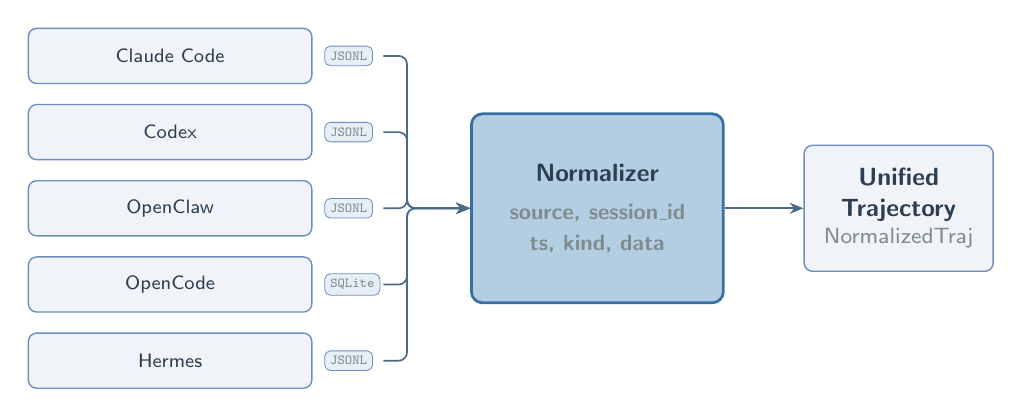
\begin{tikzpicture}

  % === Left column: 5 agent sources ===
  \node[srcbox] (s1) {Claude Code};
  \node[srcbox, below=0.25cm of s1] (s2) {Codex};
  \node[srcbox, below=0.25cm of s2] (s3) {OpenClaw};
  \node[srcbox, below=0.25cm of s3] (s4) {OpenCode};
  \node[srcbox, below=0.25cm of s4] (s5) {Hermes};

  % Badges (format labels) on the right edge of each source
  \node[badge, anchor=west] at ([xshift=0.15cm]s1.east) {\texttt{JSONL}};
  \node[badge, anchor=west] at ([xshift=0.15cm]s2.east) {\texttt{JSONL}};
  \node[badge, anchor=west] at ([xshift=0.15cm]s3.east) {\texttt{JSONL}};
  \node[badge, anchor=west] at ([xshift=0.15cm]s4.east) {\texttt{SQLite}};
  \node[badge, anchor=west] at ([xshift=0.15cm]s5.east) {\texttt{JSONL}};

  % === Center: Normalizer ===
  \coordinate (srcMid) at ($(s1.east)!0.5!(s5.east)$);
  \node[novelmodule, right=2.0cm of srcMid, minimum height=2.4cm, minimum width=3.2cm] (norm) {%
    \textbf{Normalizer}\\[3pt]
    \textcolor{textLight}{\footnotesize source, session\_id}\\
    \textcolor{textLight}{\footnotesize ts, kind, data}};

  % === Right: Unified output ===
  \node[iobox, right=1.0cm of norm, minimum height=1.6cm, minimum width=2.4cm] (out) {%
    \textbf{Unified}\\
    \textbf{Trajectory}\\[-1pt]
    \textcolor{textLight}{\footnotesize NormalizedTraj}};

  % === Arrows: sources -> normalizer ===
  \foreach \s in {s1,s2,s3,s4,s5} {
    \draw[stdarrow, rounded corners=3pt] ([xshift=0.9cm]\s.east) -- ([xshift=1.2cm]\s.east) |- (norm.west);
  }

  % Arrow: normalizer -> output
  \draw[stdarrow] (norm) -- (out);

\end{tikzpicture}
\end{document}
